\documentclass[a4paper]{article}

\usepackage{mathrsfs}
% ============================================
%         General Packages
% ============================================
\usepackage{balance}

\usepackage{kotex}      % for Korean
\usepackage{lipsum}     % for dummy text
\usepackage{array}

\usepackage{cite}   % for citation

\usepackage{amsmath,amsfonts}
\usepackage{amssymb}
\usepackage{soul}
\usepackage{mathrsfs}

\usepackage{hyperref}

    \hypersetup{
        pdftoolbar=false,        	% show Acrobat’s toolbar?
        pdfmenubar=false,        	% show Acrobat’s menu?
        pdffitwindow=false,     	% window fit to page when opened
        pdfstartview={FitH},    	% fits the width of the page to the window
        pdftitle={},    	% title
        pdfauthor={},     	% author
        %     pdfsubject={},   	% subject of the document
        %     pdfcreator={},   	% creator of the document
        %     pdfproducer={}, 	% producer of the document
        %     pdfkeywords={keyword1, key2, key3}, % list of keywords
        %     pdfnewwindow=true,      	% links in new PDF window
        colorlinks=true,       	% false: boxed links; true: colored links
        linkcolor=blue,          	% color of internal links (change box color with linkbordercolor)
        citecolor=blue,       	% color of links to bibliography
        filecolor=blue,      	% color of file links
        urlcolor=blue		% color of external links
    }

\usepackage{algorithm}
\usepackage{algorithmic}

\usepackage{epsfig}
\usepackage[dvipsnames]{xcolor}

% MY PACKAGES ===================================

\usepackage{svg}
\usepackage{subfig}

\usepackage{textcomp}
\usepackage{stfloats}
\usepackage{url}
\usepackage{verbatim}
\usepackage{graphicx}
\usepackage{multirow}
\usepackage{multicol}

\let\proof\relax
\let\endproof\relax
\usepackage{amsthm}
\usepackage{lipsum}
\usepackage{tikz}

% 
\usepackage{titlepic}
\usepackage{pdfpages}
\usepackage{etoolbox} % 조건문을 쓰기 위한 패키지


\titlepic{%
  
\includegraphics[height = 8mm]{figures/logo_KAIST_simple.png}
  \hspace{5mm}
  
\includegraphics[height = 8mm]{figures/MIC_Logo.png}
  }

% ========================================
%         TITLE and AUTHORS
% ========================================
\title{
  Neuro-Adaptive Control
}

\author{
    Myeongseok Ryu
    \thanks{\href{https://kaist-mic-lab.github.io/members/msRyu/}{Myeongseok Ryu} is Ph.D. student at KAIST, {\tt\small dding\_98@kaist.ac.kr}}%
    , and 
    Naol Samuel Erega
    \thanks{\href{https://kaist-mic-lab.github.io/members/nsErega/}{Naol Samuel Erega} is M.S. student at KAIST, {\tt\small samuelnaol7@kaist.ac.kr}}%
}

\date{
    % 20\textsuperscript{th} March 2025
    Complied on \today
}

\begin{document}

\maketitle

% ========================================
%         Contents
% ========================================

\begin{figure}[h]
  \centering
  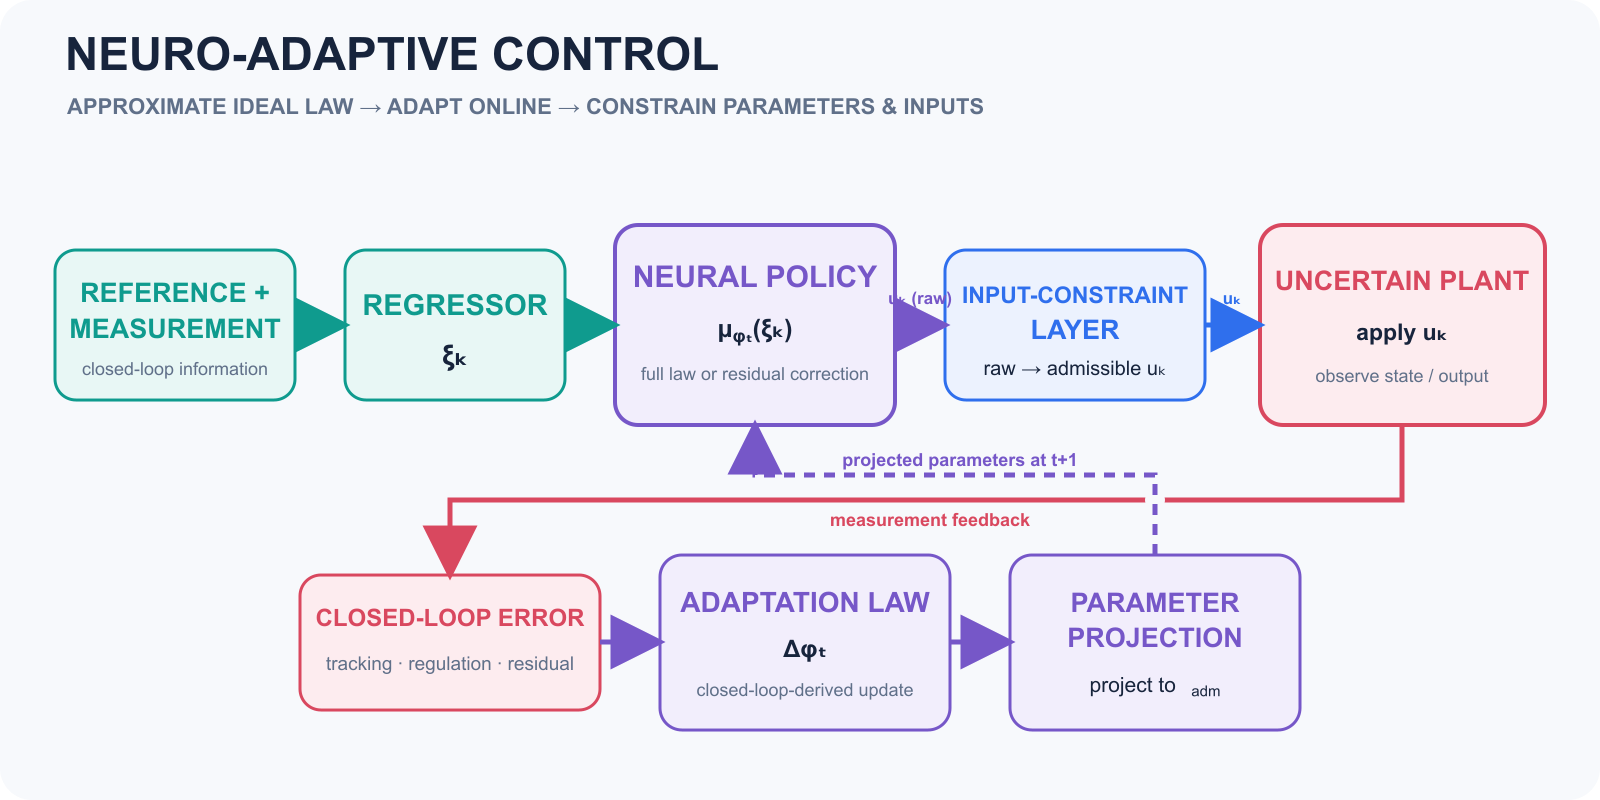
\includegraphics[width=\textwidth]{figures/07_neuro_adaptive_control.png}
  \caption{An uncertain ideal control law is represented by a neural policy whose parameters are adapted online under closed-loop and constraint conditions.}
\label{fig:}
\end{figure}


\nocite{*} % <------------ 인용있으면 삭제

Physical interaction is indexed by $k$, whereas neural-policy updates are
indexed by $t$; the two clocks need not advance at the same rate. Here $t(k)$
is the latest neural-policy update available at physical step $k$, and $k(t)$
is the latest physical sample available at learner update $t$. $\phi_t$
denotes the policy parameter available before update $t$, and $\phi_{t+1}$
denotes the updated parameter.

\section{Problem definition}

\href{https://kaist-mic-lab.github.io/research/research_themes/00_online_learning_based_optimal_control/}{Online Learning-Based Optimal Control} defines the desired policy through Bellman optimality when the decision problem and required information are available. Neuro-Adaptive Control addresses a related but distinct situation: system uncertainty prevents direct implementation of the ideal feedback law required for a declared tracking, regulation, or stabilization objective.

Consider
\begin{equation}
  x_{k+1}=f(x_k,u_k,w_k),
  \qquad
  y_k=h(x_k)+v_k
  ,
\end{equation}
where $x_k$, $u_k$, and $y_k$ are the state, control input, and measurement; $f$ and $h$ are the state-transition and measurement maps; $w_k$ represents process uncertainty or a disturbance; and $v_k$ is measurement noise. When $x_k$ is not measured, $\widehat x_k$ denotes its estimate. The dynamics may contain unknown nonlinearities or uncertain parameters. The unavailable target is first written as the ideal feedback law
\begin{equation}
  u_k^{\mathrm{ideal}}=\mu_{\mathrm{ideal}}(x_k).
\end{equation}

Neuro-Adaptive Control then \textbf{parameterizes and approximates} this law with a selected neural function class:
\begin{equation}
  \mu_{\mathrm{ideal}}(x)
  =
  \mu_{\phi^\star}(x)
  +
  \varepsilon_{\mathrm{app}}(x).
\end{equation}

The implemented policy and its online adaptation are
\begin{equation}
  \begin{aligned}
    u_k
    &=
    \mu_{\phi_{t(k)}}(\widehat x_k),\\
    \phi_t
    &\xrightarrow{\text{online adaptation}}
    \phi_{t+1}.
  \end{aligned}
\end{equation}

Here $\phi^\star$ is an ideal parameter in the chosen neural class, $\varepsilon_{\mathrm{app}}$ is its approximation error, and $\phi_t$ is the deployed parameter at learner update $t$. The law $\mu_{\mathrm{ideal}}$ is Bellman-optimal only when that connection is explicitly established.

If the controller uses a recurrent or other sequence-processing network, replace $\widehat x_k$ by a declared history-dependent information vector $\xi_k$. The network may approximate the complete feedback law or a residual correction $u_k=u_{\mathrm{nom},k}+\mu_{\phi_{t(k)}}(\xi_k)$.

Direct approximation of $\mu_{\mathrm{ideal}}$ folds the control effect of
uncertain dynamics into the policy. It does not automatically identify a
reusable model $\widehat f$.

Within the overview taxonomy, this Theme is placed in the joint
control–identification lane because closed-loop information about uncertainty
directly changes the controller. This placement does not mean that a reusable
dynamics model is identified.

\section{Why this problem matters}

The exact stabilizing or performance-improving feedback often depends on nonlinearities, disturbances, and parameters that are not available to a nominal controller. A neural function class can represent richer compensation than a fixed low-dimensional adaptive law and can update during operation.

Direct-law approximation may also avoid the full sequence of identifying a physical model and then redesigning the controller. Its primary benefit, however, is closed-loop uncertainty compensation. Without explicit mechanisms for coverage, memory, or retention, it remains closer to adaptation along the visited trajectory than to task-wide policy learning.

\section{Key challenges}

\begin{itemize}
  \item Ideal-law approximation and information: the approximation domain, $\varepsilon_{\mathrm{app}}$, available state or history information, and estimator error must be declared.
  \item Closed-loop adaptation versus learning: changing $\phi_t$ changes both the applied input and future data, while a trajectory-local update need not recover $\phi^\star$ or produce a reusable task-wide policy.
  \item Stability and constraints: bounded tracking error, bounded neural weights, admissible control inputs, and state safety are different claims.
  \item Excitation and online implementation: weak excitation can prevent parameter convergence, and sensitivity calculation, memory, and update time must remain compatible with the physical control rate.
\end{itemize}

\section{A conventional approach — Lyapunov-derived neuro-adaptation}

A conventional neuro-adaptive controller derives its parameter update from declared closed-loop error dynamics and a Lyapunov argument. Schematically,

\begin{equation}
  \begin{aligned}
    u_k
    &=
    \mu_{\phi_{t(k)}}(\widehat x_k),\\
    \phi_{t+1}
    &=
    \Pi_{\Phi_{\mathrm{adm}}}
    \left[
    \phi_t+
    \Delta\phi_t
    \!\left(e_{k(t)},\widehat x_{k(t)}\right)
    \right],
  \end{aligned}
\end{equation}

where $e_k$ is the selected tracking or regulation error and $\Delta\phi_t$ is the update derived for the specific plant and controller. The projection $\Pi_{\Phi_{\mathrm{adm}}}$ is included only when the implemented method uses an admissible parameter set.

Under its stated approximation, gain, excitation, and initialization conditions, such an update may establish boundedness of selected closed-loop signals. It need not recover $\phi^\star$, learn a globally reusable policy, or enforce actuator and state constraints.

\section{A constrained direction — optimization-based neuro-adaptation}

A constrained formulation makes the online performance objective and admissibility conditions explicit. Let $k_t:=k(t)$ denote the newest physical sample available at learner update $t$:

\begin{equation}
  \begin{aligned}
    \min_{\phi}\quad
    &\mathcal L_{\mathrm{cl},t}(\phi)\\
    \text{s.t.}\quad
    &c_{\phi,j}(\phi)\le 0,
    \qquad j=1,\ldots,n_\phi,\\
    &c_{u,i}
    \!\left(
    \mu_\phi(\widehat x_{k_t}),
    \widehat x_{k_t}
    \right)
    \le 0,
    \qquad i=1,\ldots,n_u .
  \end{aligned}
\end{equation}

$\mathcal L_{\mathrm{cl},t}$ is a closed-loop error or performance objective;
it is not a supervised loss against the unavailable
$\mu_{\mathrm{ideal}}$. Its
dependence on a candidate $\phi$ must be supplied by a declared sliding-window
or rollout prediction, forward sensitivity, or differentiable instantaneous
surrogate. Previously observed errors alone are constant with respect to a new
candidate $\phi$ and therefore do not define the displayed optimization.
Example constraints include

\begin{equation}
  c_{\phi,\ell}(\phi)
  =
  \|\phi_\ell\|_2^2-\bar\phi_\ell^2
  \le 0,
  \qquad
  c_u(\phi;\widehat x_{k_t})
  =
  \|\mu_\phi(\widehat x_{k_t})\|_2^2-\bar u^2
  \le 0.
\end{equation}

$n_\phi$ and $n_u$ count the declared parameter and input constraints,
$\phi_\ell$ is a selected parameter group, and
$\bar\phi_\ell,\bar u>0$ are prescribed bounds.

The input constraint $c_u$ is evaluated on the policy output at the current
operating condition and can directly encode input amplitude or norm. An input
rate constraint additionally requires the previous applied input, and an
energy constraint requires an accumulated or horizon state. If the implemented
actuator includes saturation or a separate safety filter, the constraint and
analysis must refer to the input actually applied to the system, not only the
raw neural-policy output.

Let $c_j$ enumerate the declared parameter constraints $c_{\phi,j}$ and
applied-input constraints $c_{u,i}$ after any required state augmentation. A
conceptual primal--dual realization takes online steps toward the constrained
target:

\begin{equation}
  \begin{aligned}
    \mathscr L_t(\phi,\lambda)
    &=
    \mathcal L_{\mathrm{cl},t}(\phi)
    +
    \sum_j\lambda_jc_j(\phi;\widehat x_{k_t}),\\
    \phi_{t+1}
    &=
    \phi_t-\eta_{\phi,t}
    \nabla_\phi\mathscr L_t(\phi_t,\lambda_t),\\
    \lambda_{j,t+1}
    &=
    \left[
    \lambda_{j,t}
    +
    \eta_{\lambda_j,t}
    c_j(\phi_t;\widehat x_{k_t})
    \right]_+ .
  \end{aligned}
\end{equation}

Here $\lambda_{j,0}\ge0$,
$\eta_{\phi,t},\eta_{\lambda_j,t}>0$, and $[\cdot]_+$ denotes projection onto
the nonnegative reals. Transient primal--dual iterates need not be feasible;
when every applied action must satisfy its constraints, an implemented
projection, safety filter, saturation, or fallback and a corresponding
closed-loop analysis remain necessary.

The \href{https://kaist-mic-lab.github.io/publications/2025-CONAC-Robot/}{\textbf{Constrained Optimization-Based Neuro-Adaptive Control (CoNAC)}}
preprint is a concrete related instance for uncertain Euler--Lagrange systems.
It uses a DNN to approximate an ideal stabilizing law and formulates online
weight adaptation with weight-norm and input constraints. The preprint reports
bounded tracking errors and DNN weights under its stated assumptions, together
with comparative numerical simulations. The scope of these guarantees is
determined by the plant, network, feasibility, and adaptation assumptions stated
in that work; extensions to other systems or architectures require corresponding
analysis.

Evidence should distinguish tracking-error boundedness, weight boundedness,
constraint satisfaction, parameter or KKT convergence, control effort,
computation time, and performance outside the theorem conditions.

\section{Application domains}

\begin{itemize}
  \item \textbf{Uncertain nonlinear vehicle and mobility subsystems} requiring
  online compensation under actuator limits.
  \item \textbf{Robotic and Euler--Lagrange systems}, including manipulators and
  motion platforms with tracking objectives.
  \item \textbf{Electric drives and mechatronic systems} subject to torque,
  current, voltage, or other input constraints.
  \item \textbf{Full-law or residual neural control} when a reusable physical
  model is unavailable or impractical to maintain online.
\end{itemize}

\section{References}

\begin{itemize}
  \item 
    \href{
      https://kaist-mic-lab.github.io/publications/2025-CONAC-Robot/
    }{
      M. Ryu, D. Hong, and K. Choi, ``Constrained Optimization-Based
  Neuro-Adaptive Control (CoNAC) for Uncertain Euler--Lagrange Systems Under
  Weight and Input Constraints,'' TechRxiv preprint, v1, 2024.
    }
\end{itemize}

% ========================================
%         Appendix
% ========================================

% \begin{appendices}
% \end{appendices}

\addcontentsline{toc}{chapter}{Bibliography}
\bibliographystyle{IEEEtran}
\bibliography{refs}

\end{document}
